\documentclass[conference]{IEEEtran}
\IEEEoverridecommandlockouts
\usepackage{cite}
\usepackage{amsmath,amssymb,amsfonts}
\usepackage{algorithmic}
\usepackage{graphicx}
\usepackage{textcomp}
\usepackage{xcolor}
\usepackage{url}
\usepackage{tikz}
\usetikzlibrary{arrows.meta,positioning}
\def\BibTeX{{\rm B\kern-.05em{\sc i\kern-.025em b}\kern-.08em
    T\kern-.1667em\lower.7ex\hbox{E}\kern-.125emX}}

\begin{document}

\title{Dual-Learning Adaptive Large Neighborhood Search for One-Dimensional Bin Packing:\\
Online Operator Selection and Offline Learned Repair}

\author{
\IEEEauthorblockN{Mohamed El Amine Kherroubi, Rayan Boukakiou, Idriss Yacine Ziadi, Idris Himeur, Adem Abdelhafidh Diar}
\IEEEauthorblockA{\textit{Higher National School of Computer Science (ESI)}\\
Algiers, Algeria}
}

\maketitle

\begin{abstract}
The one-dimensional bin packing problem (1D-BPP) is a strongly NP-hard
combinatorial optimization problem in which a set of weighted items must be
packed into the fewest identical capacity-limited bins. Metaheuristics scale to
large instances but rely on hand-designed operators and fixed policies that do
not adapt to the state of the search. We present a dual-learning Adaptive Large
Neighborhood Search (ALNS) that injects machine learning at two distinct decision
points of a single search loop: an \emph{online} warm-start contextual bandit
(LinUCB) selects the destroy operator from a five-dimensional search-state
context, while an \emph{offline} gradient-boosted-trees model, trained by
behavioral cloning of Best-Fit Decreasing, ranks feasible bins during repair. An
ablation study isolates the contribution of each learning component, and a
multi-dataset evaluation on standard benchmarks (Scholl, Falkenauer, W\"ascher,
Hard28) characterizes the combined method. On the Scholl-2 slice, online operator
selection alone closes the mean optimality gap (from $0.20$ to $0.00$ bins) at
negligible cost, whereas the offline repair model adds computation without
improving quality on this easy slice---an ablation finding that motivates learned
repair for harder instances.
\end{abstract}

\begin{IEEEkeywords}
bin packing, adaptive large neighborhood search, contextual bandit, LinUCB,
gradient boosting, hyper-heuristics, machine learning, combinatorial optimization
\end{IEEEkeywords}

\section{Introduction}\label{sec:intro}

The one-dimensional bin packing problem (1D-BPP) is a classical combinatorial
optimization problem with broad industrial relevance, from logistics and
cutting-stock to scheduling and cloud resource allocation. Given $n$ items, each
with a positive integer size, and an unlimited supply of identical bins of fixed
capacity $C$, the task is to assign every item to a bin without exceeding capacity
while using as few bins as possible. Despite its simple statement, 1D-BPP is
strongly NP-hard~\cite{bGarey}, so exact solvers do not scale to large instances
and practitioners rely on heuristics and metaheuristics.

Two families dominate practical 1D-BPP solving. Constructive heuristics such as
First-Fit Decreasing (FFD) and Best-Fit Decreasing (BFD) run in $O(n\log n)$ and
offer bounded worst-case guarantees---FFD uses at most $\tfrac{11}{9}\,\mathrm{OPT}+\tfrac{6}{9}$
bins~\cite{bJohnson}---but they produce a single deterministic packing with no
further improvement. Metaheuristics---simulated annealing~\cite{bKirkpatrick},
tabu search~\cite{bGlover}, grouping genetic algorithms~\cite{bFalkenauer}, and
ant colony optimization~\cite{bDorigo}---explore the solution space iteratively
and reach higher-quality packings on hard instances. Their effectiveness,
however, hinges on manually designed neighborhood operators and on
selection and acceptance policies whose parameters are fixed in advance and
applied identically to every instance and at every stage of the search.
Crucially, classical metaheuristics do not exploit the information generated
during the search itself: neither the time-varying usefulness of an operator nor
the structural regularities of good placements are ever learned.

Machine learning (ML) offers a principled way to make these decisions
data-driven. Following the taxonomy of Bengio \textit{et al.}~\cite{bBengio}, ML
can be hybridized with metaheuristics in three broad modes: (i) predicting
algorithm configuration or parameters offline, (ii) guiding search decisions
online from the current state, and (iii) replacing a hand-crafted operator with a
learned model. The first mode adapts poorly within a single run, and the third
can be data- and compute-intensive in isolation. We therefore combine the second
and third modes at the two decisions that most influence ALNS quality: which part
of the incumbent solution to destroy, and how to rebuild it.

Learning-augmented metaheuristics have shown strong results on routing and
packing problems. Reinforcement learning has been used to select low-level
heuristics in hyper-heuristic frameworks, and neural models have been embedded in
large neighborhood search---for example Neural LNS for vehicle
routing~\cite{bHottung}---to learn destruction or repair policies. Contextual
bandits, in particular LinUCB~\cite{bLi,bChu}, provide a lightweight online
mechanism for adaptive operator selection with theoretical regret guarantees,
while gradient-boosted trees~\cite{bFriedman} are strong tabular rankers
well suited to scoring candidate placements. These ingredients have rarely been
combined within a single bin-packing solver.

This paper presents a dual-learning ALNS for 1D-BPP that injects learning at both
decision points of the destroy--repair loop. First, an online warm-start LinUCB
contextual bandit selects, at every iteration, one of three destroy operators
from a five-dimensional description of the current search state. Second, an
offline gradient-boosted-trees model, trained by behavioral cloning of BFD, ranks
the feasible bins for each displaced item during repair. The two components are
independent and can be toggled separately, which lets us isolate their individual
and joint contributions through an ablation study. To our knowledge, this
two-point integration---online operator selection together with offline learned
repair---has not been reported for bin packing.

The remainder of the paper is organized as follows.
Section~\ref{sec:formulation} formalizes the problem,
Section~\ref{sec:approach} describes the dual-learning ALNS and its two learning
components, Section~\ref{sec:experiments} reports the experimental protocol, the
ablation study, and the multi-dataset and comparative results, and
Section~\ref{sec:conclusion} concludes and outlines perspectives.

\section{Problem Formulation}\label{sec:formulation}

Let $\mathcal{I}=\{1,\dots,n\}$ be a set of items with strictly positive integer
sizes $s_i\in\mathbb{Z}_{>0}$, and let identical bins have integer capacity
$C\in\mathbb{Z}_{>0}$ with $s_i\le C$ for all $i$. Using binary variables
$x_{ij}=1$ iff item $i$ is placed in bin $j$, and $y_j=1$ iff bin $j$ is used
(with $j\in\{1,\dots,n\}$), the problem is:
\begin{align}
\min \quad & \sum_{j=1}^{n} y_j \label{eq:obj}\\
\text{s.t.}\quad & \sum_{j=1}^{n} x_{ij}=1, && \forall i\in\mathcal{I} \label{eq:assign}\\
& \sum_{i=1}^{n} s_i\,x_{ij}\le C\,y_j, && \forall j \label{eq:cap}\\
& x_{ij}\le y_j,\; x_{ij},y_j\in\{0,1\}. && \label{eq:link}
\end{align}
Constraint~\eqref{eq:assign} assigns each item to exactly one bin,
\eqref{eq:cap} enforces capacity and links assignment to bin usage, and the
objective~\eqref{eq:obj} minimizes the number of bins used. A standard continuous
lower bound is
\begin{equation}
\mathrm{LB}_1=\left\lceil \frac{\sum_{i=1}^{n} s_i}{C} \right\rceil ,\label{eq:lb}
\end{equation}
which is valid because the total item volume $\sum_i s_i$ must be distributed over
bins of capacity $C$, requiring at least $\sum_i s_i / C$ of them; integrality
gives the ceiling. Sharper bounds exist, such as the $L_2$ bound of Martello and
Toth~\cite{bMartello}, but $\mathrm{LB}_1$ is sufficient as the progress indicator
used throughout this work. 1D-BPP is strongly NP-hard by reduction from
3-Partition~\cite{bGarey}, which justifies a metaheuristic treatment.

\section{Proposed Dual-Learning ALNS}\label{sec:approach}

\begin{figure}[t]
\centering
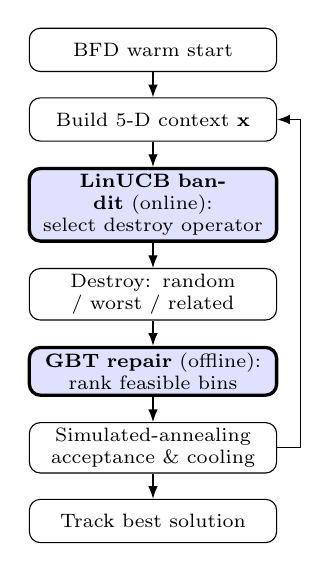
\begin{tikzpicture}[
  node distance=3.2mm,
  box/.style={draw, rounded corners, align=center, font=\scriptsize,
              minimum height=5.5mm, text width=3.0cm, inner sep=2pt},
  ml/.style={box, fill=blue!12, very thick},
  arr/.style={-{Latex[length=1.6mm]}}
]
\node[box] (start) {BFD warm start};
\node[box, below=of start] (ctx) {Build 5-D context $\mathbf{x}$};
\node[ml, below=of ctx] (bandit) {\textbf{LinUCB bandit} (online):\\ select destroy operator};
\node[box, below=of bandit] (destroy) {Destroy: random / worst / related};
\node[ml, below=of destroy] (repair) {\textbf{GBT repair} (offline):\\ rank feasible bins};
\node[box, below=of repair] (sa) {Simulated-annealing\\ acceptance \& cooling};
\node[box, below=of sa] (best) {Track best solution};
\foreach \a/\b in {start/ctx, ctx/bandit, bandit/destroy, destroy/repair, repair/sa, sa/best}
  \draw[arr] (\a)--(\b);
\draw[arr] (sa.east) -- ++(3mm,0) |- (ctx.east);
\end{tikzpicture}
\caption{Architecture of the dual-learning hybrid ALNS. Shaded boxes mark the two
machine-learning injection points; the right-hand arrow is the iteration loop.}
\label{fig:arch}
\end{figure}

\subsection{Solution Encoding and Warm Start}
A solution is the assignment of items to bins. Internally the search stores, for
each item, the index of its bin and, for each bin, its current load, so that a
removal or insertion updates in $O(1)$ and the objective---the number of
non-empty bins---is read directly. The search is warm-started with Best-Fit
Decreasing (BFD): items are processed in non-increasing size order and each is
placed in the open bin that leaves the smallest residual capacity, a new bin being
opened only when no bin can host it. A tight initial packing gives ALNS fewer bins
to eliminate and shortens the time spent recovering from a poor initialization.

\subsection{Adaptive Large Neighborhood Search}
The search follows the large-neighborhood-search paradigm~\cite{bShaw} in its
adaptive form~\cite{bRopke}. Each iteration (i) \emph{destroys} the incumbent by
removing a subset $D$ of items and (ii) \emph{repairs} the partial solution by
reinserting $D$. Because repair can produce any feasible completion, the
neighborhood is implicitly exponential in $|D|$, which allows the search to escape
local optima unreachable by single-item moves. Three destroy operators form the
portfolio: \emph{random} removal of $k$ items; \emph{worst-load} removal, which
empties the least-filled bins first; and \emph{related-item} removal, which
removes a seed item together with the items closest to it in size. The destruction
radius $k$ is drawn uniformly from $[\lfloor 0.05\,n\rfloor,\lfloor 0.25\,n\rfloor]$
and is widened toward its upper bound as stagnation grows; all operators guarantee
that at least one item remains placed, preventing total destruction.

\subsection{Acceptance: Simulated Annealing}
Candidates are accepted by simulated annealing. A candidate whose bin-count change
is $\Delta$ is accepted whenever $\Delta\le 0$, and otherwise with probability
$\exp(-\Delta/T)$. The temperature follows geometric cooling
$T\leftarrow \alpha_{\mathrm{cool}}\,T$ with $T_0=1/\ln 2$ and
$\alpha_{\mathrm{cool}}=0.9995$. To avoid premature freezing, a soft reheat lifts
$T$ back toward $0.35\,T_0$ during prolonged stagnation, and a diversification
restart---reverting to the best solution found, partially reheating to
$0.20\,T_0$, and shrinking the patience window---is triggered when no improvement
occurs within a budget of iterations. The fixed iteration budget is the sole
termination criterion.

\subsection{Online Learning: Warm-Start LinUCB Operator Selection}
Operator selection is delegated to a warm-start contextual bandit. During the
first $300$ selections, a context-free Beta--Bernoulli Thompson sampler quickly
identifies promising operators, mitigating the cold-start of a linear bandit on
short runs. Thereafter a disjoint LinUCB bandit~\cite{bChu} takes over: for a
context vector $\mathbf{x}\in\mathbb{R}^5$ it selects the operator that maximizes
\begin{equation}
\hat{\boldsymbol{\theta}}_k^\top \mathbf{x}
+ \alpha\sqrt{\mathbf{x}^\top A_k^{-1}\mathbf{x}},
\qquad \hat{\boldsymbol{\theta}}_k=A_k^{-1}\mathbf{b}_k,\label{eq:ucb}
\end{equation}
with $\alpha=0.3$, updating $A_k^{-1}$ by the $O(d^2)$ Sherman--Morrison formula
and $\mathbf{b}_k$ by $\mathbf{b}_k\leftarrow\mathbf{b}_k+r\,\mathbf{x}$. The
context encodes the normalized temperature $T/T_0$, the stagnation progress toward
the next restart, the cost-to-bound ratio $f(x)/\mathrm{LB}_1$, the destruction
radius $k/n$, and the overall search progress. The reward is
$\min(1,\,\text{bins\_saved}/\text{gap})$ when bins are saved---normalized by the
gap to $\mathrm{LB}_1$ so that improvements near the optimum count more---$0.2$ for
an accepted non-improving move, and $0$ for a rejected one.

\subsection{Offline Learning: GBT Repair by Behavioral Cloning}
Repair reinserts displaced items in non-increasing size order. For an item, the
set of feasible bins (those with enough residual capacity) is scored by a gradient
boosted classifier~\cite{bFriedman}, and the item is placed in the highest-scoring
bin; a new bin is opened only when no bin is feasible. The model is trained offline
by behavioral cloning of BFD: each feasible (item, bin) pair is labeled $1$ if BFD
would select that bin and $0$ otherwise. Every pair is encoded by eleven features
normalized by capacity or instance size---item size and its square, size rank,
fraction of items still to reinsert, bin load, residual capacity, post-placement
slack, bin occupancy, the largest and smallest item already in the bin, and the
fill ratio. Training pools two trace types---fresh BFD replays and
post-destruction repair states---to reduce the distribution shift between offline
replay and the mid-search states encountered at inference. A standard scaler is
stored with the model, and a fast predictor applies it in NumPy and reads class
probabilities directly, avoiding per-call validation overhead. Algorithm~\ref{alg:alns}
summarizes the complete loop.

\begin{figure}[t]
\centering
\begin{algorithmic}[1]
\STATE $x \leftarrow \textsc{BFD-WarmStart}()$;\; $x^\star \leftarrow x$
\FOR{$t=1$ \TO $\mathrm{max\_iter}$}
  \STATE $\mathbf{x}_{\text{ctx}} \leftarrow \textsc{Context}(x,T,t)$
  \STATE $a \leftarrow \textsc{Bandit.Select}(\mathbf{x}_{\text{ctx}})$
  \STATE $(\hat{x},D) \leftarrow \textsc{Destroy}_a(x,k)$
  \STATE $x' \leftarrow \textsc{RepairGBT}(\hat{x},D)$
  \STATE accept $x'$ by simulated annealing; update $x^\star$
  \STATE $\textsc{Bandit.Update}(a,\mathbf{x}_{\text{ctx}},r)$;\; cool/reheat $T$
\ENDFOR
\RETURN $x^\star$
\end{algorithmic}
\caption{Dual-learning hybrid ALNS.}
\label{alg:alns}
\end{figure}

\section{Experiments, Results and Analysis}\label{sec:experiments}

\subsection{Protocol and Setup}
All runs use a fixed random seed ($42$), a budget of $300$ ALNS iterations, an
initial temperature $T_0=1/\ln 2$, a cooling rate $\alpha_{\mathrm{cool}}=0.9995$,
and a single pre-trained repair model shared across every dataset. The solver is
implemented in Python~3.13 with scikit-learn~\cite{bPedregosa} for the
gradient-boosted repair model, and experiments were run on a workstation running
Windows~11 with an Intel Core i9-13950HX CPU and 64\,GB of RAM. Solution quality
is measured by the gap to the
lower bound, $\text{gap}=\text{bins used}-\mathrm{LB}_1$ of~\eqref{eq:lb}; a gap of
zero certifies optimality with respect to $\mathrm{LB}_1$.

\subsection{Datasets}
We evaluate on four widely used 1D-BPP benchmark families, summarized in
Table~\ref{tab:datasets}. Scholl-2 contains uniformly distributed instances with
capacity $1000$ and $50$--$500$ items. Falkenauer-T comprises triplet instances,
where an optimal bin holds one large and two small items, at capacity $1000$.
Falkenauer-U holds uniform instances with the tighter capacity $150$. W\"ascher
contributes hard cutting-stock-style instances at capacity $10000$, and Hard28 a
set of difficult $160$--$200$-item instances at capacity $1000$.

\begin{table}[htbp]
\caption{Benchmark datasets used in the evaluation.}
\label{tab:datasets}
\centering
\begin{tabular}{l c c l}
\hline
\textbf{Dataset} & \textbf{Capacity} & \textbf{Items} & \textbf{Structure}\\
\hline
Scholl-2      & 1000  & 50--500   & uniform \\
Falkenauer-T  & 1000  & 60--501   & triplets \\
Falkenauer-U  & 150   & 120--1000 & uniform \\
W\"ascher     & 10000 & varied    & cutting-stock \\
Hard28        & 1000  & 160--200  & hard \\
\hline
\end{tabular}
\end{table}

\subsection{Parameter Calibration}
The ALNS hyperparameters---cooling rate, destruction radii, and the reheat and
restart thresholds---were tuned with an Optuna search. The bandit uses an
exploration coefficient $\alpha=0.3$ and a $300$-call Thompson-sampling warm-up,
and the random seed is fixed so that every reported run is reproducible.

\subsection{Ablation Study}
To isolate the effect of each learning component we run four configurations on the
first five $50$-item Scholl-2 instances, keeping all ALNS settings identical and
toggling only the two switches (Table~\ref{tab:ablation},
Fig.~\ref{fig:ablation}). The no-learning
baseline---random operator choice and best-fit repair---averages $0.20$ bins above
$\mathrm{LB}_1$. Enabling only the online bandit closes the gap entirely ($0.00$),
the best of the four configurations, confirming that adaptive operator selection is
the decisive factor on this slice. The offline repair model---alone or combined
with the bandit---keeps the gap at $0.20$ while more than doubling the solve time,
so on this small, already near-optimal slice it adds cost and even slightly
degrades the online-only result. The two mechanisms thus act on different levers:
online operator selection carries the quality gain here, whereas learned repair is
expected to matter on harder instances with larger feasible-bin sets.

\begin{table}[htbp]
\caption{Ablation on Scholl-2 (50 items, 5 instances).}
\label{tab:ablation}
\centering
\begin{tabular}{l c c c c}
\hline
\textbf{Configuration} & \textbf{Avg bins} & \textbf{Avg gap} & \textbf{Fill (\%)} & \textbf{Time (s)}\\
\hline
No learning   & 18.2 & 0.20 & 92.76 & 0.153 \\
Online only   & 18.0 & 0.00 & 93.76 & 0.186 \\
Offline only  & 18.2 & 0.20 & 92.76 & 0.353 \\
Both combined & 18.2 & 0.20 & 92.76 & 0.362 \\
\hline
\end{tabular}
\end{table}

\begin{figure}[t]
\centering
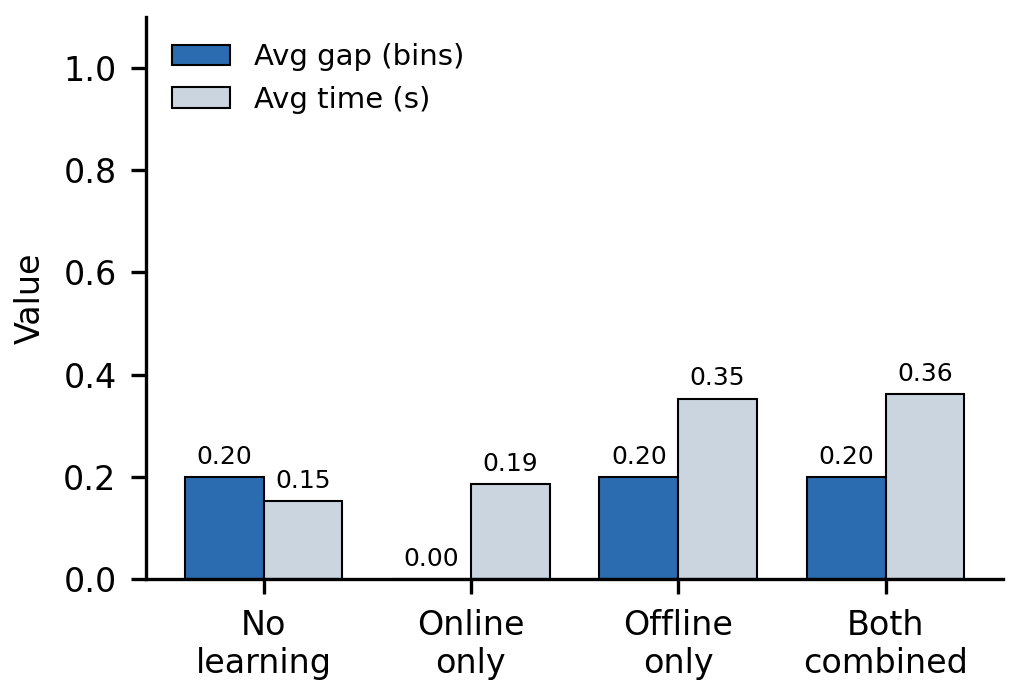
\includegraphics[width=0.92\linewidth]{figures/ablation.png}
\caption{Ablation on Scholl-2: average optimality gap and solve time per
configuration. Online operator selection removes the gap at no time cost; learned
repair roughly doubles runtime.}
\label{fig:ablation}
\end{figure}

\subsection{Multi-Dataset Results}
Table~\ref{tab:multi} reports the combined method across the five families. The
solver reaches $\mathrm{LB}_1$ or stays within one bin on the great majority of
instances: mean gaps are $0.20$ (Scholl-2), $1.00$ (Falkenauer-T), $0.20$
(Falkenauer-U), $0.60$ (W\"ascher) and $0.67$ (Hard28). The triplet instances of
Falkenauer-T are the hardest relative to $\mathrm{LB}_1$, consistent with the known
weakness of the continuous bound on triplet structures, where the true optimum
typically exceeds $\mathrm{LB}_1$ by one bin. Runtime grows with item count and
capacity, from sub-second on Scholl-2 to roughly $14$~s on the $160$-item Hard28
instances, reflecting the cost of model-guided repair over larger feasible-bin
sets.

\begin{table}[htbp]
\caption{Combined method across datasets (gap to lower bound).}
\label{tab:multi}
\centering
\begin{tabular}{l c c c}
\hline
\textbf{Dataset} & \textbf{Inst.} & \textbf{Avg gap} & \textbf{Time (s)}\\
\hline
Scholl-2 (50)      & 5 & 0.20 & 0.6--1.2 \\
Falkenauer-T (60)  & 5 & 1.00 & 1.0--1.7 \\
Falkenauer-U (120) & 5 & 0.20 & 4.3--5.8 \\
W\"ascher          & 5 & 0.60 & 1.0--2.2 \\
Hard28 (160)       & 3 & 0.67 & 13.5--15.1 \\
\hline
\end{tabular}
\end{table}

\subsection{Comparative Study}
Table~\ref{tab:compare} compares the dual-learning ALNS with classical baselines
implemented in the same framework, all run in a single session on the hardware
above so that runtimes are directly comparable. Exact methods (branch-and-bound,
dynamic programming) are omitted because they are intractable at $n=50$. The pure
constructive heuristics FFD and BFD are instantaneous but leave a mean gap of
$1.80$ bins, and the standalone trajectory metaheuristics---simulated annealing
and tabu search---do not improve on construction within their default budgets on
this slice. The population methods are stronger but costly and stochastic: the
genetic algorithm reaches a gap of $1.00$, and ant colony optimization reaches the
optimal gap ($0.00$) at roughly $8\times$ the runtime of our method ($3.03$\,s
versus $0.36$\,s). The dual-learning ALNS attains a stable, deterministic gap of
$0.20$ in $0.36$\,s, outperforming the constructive, trajectory, and genetic
baselines on quality and approaching ant colony optimization at a fraction of its
cost. The metaheuristic baselines are stochastic, so their gaps vary across runs;
a single aligned run is reported.

\begin{table}[htbp]
\caption{Comparison on Scholl-2 (50 items, 5 instances): mean gap to $\mathrm{LB}_1$ and mean solve time.}
\label{tab:compare}
\centering
\begin{tabular}{l c c}
\hline
\textbf{Method} & \textbf{Avg gap} & \textbf{Time (s)}\\
\hline
FFD / BFD            & 1.80 & $<0.01$ \\
Simulated annealing  & 1.80 & 0.21 \\
Tabu search          & 1.80 & 0.13 \\
Genetic algorithm    & 1.00 & 0.82 \\
Ant colony           & 0.00 & 3.03 \\
\textbf{Dual-learning ALNS} & \textbf{0.20} & \textbf{0.36} \\
\hline
\end{tabular}
\end{table}

\section{Conclusion and Perspectives}\label{sec:conclusion}
We presented a dual-learning Adaptive Large Neighborhood Search for the
one-dimensional bin packing problem that injects machine learning at two decision
points of the destroy--repair loop: an online warm-start LinUCB bandit for
destroy-operator selection and an offline gradient-boosted repair model trained by
behavioral cloning of Best-Fit Decreasing. An ablation isolating the two
components shows that online operator selection is the decisive, low-cost
component---it removes the optimality gap on the Scholl-2 slice at negligible
runtime---while the offline repair model did not improve quality on this easy slice
and added computation, a candid ablation finding. Across four standard benchmark
families the combined method nonetheless stays within one bin of the lower bound on
most instances. The main limitations are the small evaluation slices, the
single-run reporting of stochastic baselines, and the runtime overhead of the
offline model. Future work will extend the evaluation to full datasets and stronger
lower bounds such as the Martello--Toth $L_2$ bound, where learned repair is
expected to pay off on larger feasible-bin sets, replace the cloned repair model
with a policy learned directly from search reward, and study the transfer of the
learned components across instance families.

\begin{thebibliography}{00}
\bibitem{bCoffman} E. G. Coffman, M. R. Garey, and D. S. Johnson, ``Approximation algorithms for bin packing: a survey,'' in \textit{Approximation Algorithms for NP-Hard Problems}, 1996, pp. 46--93.
\bibitem{bDelorme} M. Delorme, M. Iori, and S. Martello, ``Bin packing and cutting stock problems: Mathematical models and exact algorithms,'' \textit{Eur. J. Oper. Res.}, vol. 255, no. 1, pp. 1--20, 2016.
\bibitem{bJohnson} D. S. Johnson, ``Near-optimal bin packing algorithms,'' Ph.D. dissertation, MIT, Cambridge, MA, 1973.
\bibitem{bGarey} M. R. Garey and D. S. Johnson, \textit{Computers and Intractability: A Guide to the Theory of NP-Completeness}. San Francisco, CA: Freeman, 1979.
\bibitem{bMartello} S. Martello and P. Toth, \textit{Knapsack Problems: Algorithms and Computer Implementations}. New York, NY: Wiley, 1990.
\bibitem{bKirkpatrick} S. Kirkpatrick, C. D. Gelatt, and M. P. Vecchi, ``Optimization by simulated annealing,'' \textit{Science}, vol. 220, no. 4598, pp. 671--680, 1983.
\bibitem{bGlover} F. Glover, ``Future paths for integer programming and links to artificial intelligence,'' \textit{Comput. Oper. Res.}, vol. 13, no. 5, pp. 533--549, 1986.
\bibitem{bFalkenauer} E. Falkenauer, ``A hybrid grouping genetic algorithm for bin packing,'' \textit{J. Heuristics}, vol. 2, no. 1, pp. 5--30, 1996.
\bibitem{bDorigo} M. Dorigo and T. St\"utzle, \textit{Ant Colony Optimization}. Cambridge, MA: MIT Press, 2004.
\bibitem{bShaw} P. Shaw, ``Using constraint programming and local search methods to solve vehicle routing problems,'' in \textit{Proc. Int. Conf. Principles and Practice of Constraint Programming (CP)}, 1998, pp. 417--431.
\bibitem{bRopke} S. Ropke and D. Pisinger, ``An adaptive large neighborhood search heuristic for the pickup and delivery problem with time windows,'' \textit{Transp. Sci.}, vol. 40, no. 4, pp. 455--472, 2006.
\bibitem{bLi} L. Li, W. Chu, J. Langford, and R. E. Schapire, ``A contextual-bandit approach to personalized news article recommendation,'' in \textit{Proc. 19th Int. Conf. World Wide Web (WWW)}, 2010, pp. 661--670.
\bibitem{bChu} W. Chu, L. Li, L. Reyzin, and R. E. Schapire, ``Contextual bandits with linear payoff functions,'' in \textit{Proc. 14th Int. Conf. Artificial Intelligence and Statistics (AISTATS)}, 2011, pp. 208--214.
\bibitem{bFriedman} J. H. Friedman, ``Greedy function approximation: a gradient boosting machine,'' \textit{Ann. Statist.}, vol. 29, no. 5, pp. 1189--1232, 2001.
\bibitem{bBengio} Y. Bengio, A. Lodi, and A. Prouvost, ``Machine learning for combinatorial optimization: a methodological tour d'horizon,'' \textit{Eur. J. Oper. Res.}, vol. 290, no. 2, pp. 405--421, 2021.
\bibitem{bHottung} A. Hottung and K. Tierney, ``Neural large neighborhood search for the capacitated vehicle routing problem,'' in \textit{Proc. 24th Eur. Conf. Artificial Intelligence (ECAI)}, 2020, pp. 443--450.
\bibitem{bScholl} A. Scholl, R. Klein, and C. J\"urgens, ``BISON: A fast hybrid procedure for exactly solving the one-dimensional bin packing problem,'' \textit{Comput. Oper. Res.}, vol. 24, no. 7, pp. 627--645, 1997.
\bibitem{bSchwerin} P. Schwerin and G. W\"ascher, ``The bin-packing problem: A problem generator and some numerical experiments with FFD packing and MTP,'' \textit{Int. Trans. Oper. Res.}, vol. 4, no. 5--6, pp. 377--389, 1997.
\bibitem{bPedregosa} F. Pedregosa \textit{et al.}, ``Scikit-learn: Machine learning in Python,'' \textit{J. Mach. Learn. Res.}, vol. 12, pp. 2825--2830, 2011.
\end{thebibliography}

\end{document}
